\def\pgfsysdriver{pgfsys-dvisvgm.def}
\documentclass[dvisvgm,tikz,border=10pt]{standalone}
\usepackage{tikz}
\usepackage{amsmath}
\usetikzlibrary{arrows.meta,patterns,positioning}
\tikzset{
 clause/.style={rectangle,draw=black,fill=white,minimum size=7mm,line width=.9pt},
 varnode/.style={circle,draw=black,minimum size=9mm,line width=.9pt},
 truevar/.style={varnode,fill=white},
 falsevar/.style={varnode,fill=gray!55},
 freevar/.style={varnode,pattern=north east lines,pattern color=gray!65},
 positive/.style={draw=black,line width=1pt},
 negative/.style={positive,dash pattern=on 4pt off 3pt},
 every node/.style={text=black,font=\sffamily},
}

\begin{document}
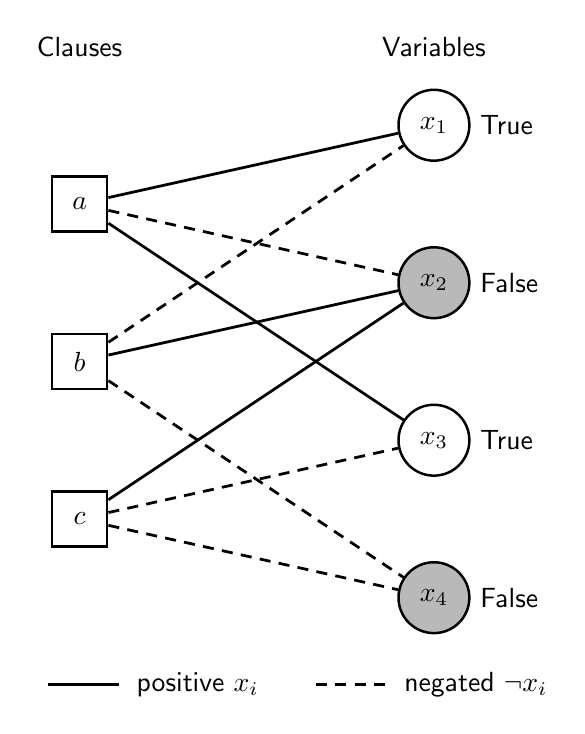
\begin{tikzpicture}
\node at (0,4) {Clauses}; \node at (4.5,4) {Variables};
\node[clause] (a) at (0,2) {$a$};
\node[clause] (b) at (0,0) {$b$};
\node[clause] (c) at (0,-2) {$c$};
\node[truevar,label=right:True] (x1) at (4.5,3) {$x_1$};
\node[falsevar,label=right:False] (x2) at (4.5,1) {$x_2$};
\node[truevar,label=right:True] (x3) at (4.5,-1) {$x_3$};
\node[falsevar,label=right:False] (x4) at (4.5,-3) {$x_4$};
\draw[positive] (a)--(x1); \draw[negative] (a)--(x2);
\draw[positive] (a)--(x3); \draw[negative] (b)--(x1);
\draw[positive] (b)--(x2); \draw[negative] (b)--(x4);
\draw[positive] (c)--(x2); \draw[negative] (c)--(x3);
\draw[negative] (c)--(x4);
\draw[positive] (-.4,-4.1)--(.5,-4.1);
\node[anchor=west] at (.6,-4.1) {positive $x_i$};
\draw[negative] (3,-4.1)--(3.9,-4.1);
\node[anchor=west] at (4,-4.1) {negated $\neg x_i$};
\end{tikzpicture}
\end{document}
